\capitulo{4}{Técnicas y herramientas}

En este capítulo se encuentran las técnicas y herramientas utilizadas en el proceso de \textbf{investigación}, la creación del \textbf{servicio web} además de una sección con las \textbf{herramientas generales} usadas en todo el proyecto.

\section{Investigación}

El proyecto ha sido desarrollado aplicando diversas técnicas de minería de datos siguiendo el proceso KDD~\cite{ubu:mineria1} (Fig.~\ref{fig:kdd}). Aunque en esta memoria se explicará superficialmente, el desarrollo completo de la investigación se encuentra en el cuaderno de investigación adjuntado.

\begin{figure}
	\centering
	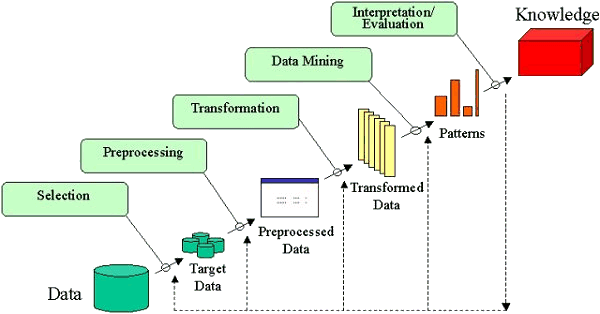
\includegraphics[width=\linewidth]{kdd}
	\caption{Flujo KDD~\cite{fayyad1996data}.}
	\label{fig:kdd}
\end{figure}

Para el proceso del clasificador final el flujo KDD ha sido el siguiente:

\begin{enumerate}
	\item \textbf{Selección}
		Los datos han sido cedidos por la asociación abulense \textit{PRONISA} que contiene jornadas nocturnas con identificadores de la cama, datos de presiones y datos vitales. Estos datos no están balanceados ya que existe una mayor cantidad de datos del paciente durmiendo que bajo una crisis epiléptica.
	\item \textbf{Preprocesado}
		Los datos se han limpiado reduciendo ruidos mediante filtros de señal.
	\item \textbf{Transformación}
		Se han generado datos estadísticos para series temporales que optimizaban el valor del área bajo la curva PCR~\cite{saito2015precision} desde los datos preprocesados.
	\item \textbf{Minería de datos}
		Se ha aplicado un sistema de clasificación doble, en primer lugar se utiliza un árbol de clasificación muy simple que divide entre las situaciones de despierto (bajas presiones en la cama) y acostado, en esta situación se aplica un clasificador \textit{Random Forest}~\cite{breiman2001random} para determinar si hay crisis o no.
	\item \textbf{Interpretación}
		Se ha desplegado una aplicación web con datos en tiempo real para evaluar de manera constante la situación actual del paciente.
\end{enumerate}

Este proceso de investigación se realizó sobre \textit{Python} utilizando el ecosistema de bibliotecas \textit{SciPy}~\cite{tool:scipy}, la biblioteca homónima se usó para crear filtros sobre los datos.

\paragraph{\textit{scikit-learn}~\cite{tool:scikit-learn}}biblioteca con funciones de aprendizaje automático para la creación de nuestros modelos.
\paragraph{\textit{NumPy}~\cite{tool:numpy}}biblioteca de computación especialmente útil para el almacenamiento de los datos y sus operaciones.
\paragraph{\textit{Pandas}~\cite{tool:pandas}}biblioteca de análisis de datos que usamos para almacenar los datos cargados desde los ficheros \textit{csv}.
\paragraph{\textit{MatPlotLib}~\cite{tool:matplotlib}}herramienta de dibujado usada para representar los datos y sus proyecciones.

Además, en algunas partes de la investigación se utilizó \textit{Weka}~\cite{tool:weka} para estudiar métodos que no se encontraban en \textit{scikit-learn} como el \textit{Random Balance}~\cite{diez2015random} o \textit{Rotation Forest}~\cite{rodriguez2006rotation}.

\section{Servicio web}

\subsection{\textit{Backend}}

Las herramientas utilizadas para programar el servidor han sido las siguientes:
\paragraph{Flask~\cite{tool:flask}}\textit{Microframwork} de código abierto (BSD) que ofrece una capa de abstracción muy alta de un servicio web, se utiliza para la creación de la lógica de negocio mediante la gestión de las rutas.
\paragraph{Jinja~\cite{tool:jinja}}Gestor de plantillas de código abierto (BSD) para Python, se utiliza para la creación de la interfaz web mediante la creación de páginas dinámicas en HTML.
\paragraph{Flask-SocketIO~\cite{tool:flask-socketio}}Integración del servicio de \textit{sockets}, \textit{Socket.IO}~\cite{tool:socketio}, compatible con los \textit{WebSockets}, se utiliza para la difusión de los datos en pacientes.
\paragraph{Gevent y Eventlet~\cite{tool:eventlet, tool:gevent}}Bibliotecas para el uso de tiempo real, asíncrono de hilos para el uso de \textit{Socket.IO}, el uso de estas bibliotecas es facilitar el procesado y difusión en tiempo real de los datos de los pacientes. 

Para la programación del sistema de hilos que distribuyen datos en tiempo real se siguieron los paradigmas de la programación orientada a objetos y de programación funcional. El sistema de rutas siguió las guías del \textit{microframework Flask}. 

Algunos patrones de diseño utilizados han sido el \textit{Singleton} para la API así como un \textit{Proxy} entre la interfaz web y la lógica de el API.

\subsection{\textit{Frontend}}

Para el desarrollo de la parte visible de la aplicación se han usado otra serie de herramientas:
\paragraph{Bootstrap~\cite{wiki:boostrap}}\textit{Framework} de \textit{CSS} de código abierto (MIT) creado por \textit{Twitter} para la creación de aplicaciones web redimensionables. Todos los estilos de la web se apoyan en este \textit{framework}.
\paragraph{jQuery~\cite{wiki:jquery}}\textit{Framework} de \textit{JavaScript} de código abierto (MIT) que simplifica el acceso al \textit{HTML DOM} de la página. La gestión de los eventos de la web se gestionan mediante este \textit{framework}.
\paragraph{Chart.js}Biblioteca de \textit{JavaScript} de código abierto (MIT) para la creación de grafos en \texttt{canvas}. Se usa para la visualización de las gráficas de presiones y constantes vitales.

\section{Herramientas generales}

Para el desarrollo general del proyecto se han utilizado las siguientes herramientas según el ámbito al que pertenecen:

\subsubsection{Servidor}
\paragraph{\textit{Nginx}}servidor web y de proxy reverso ligero de alto rendimiento~\cite{wiki:nginx} de código abierto (BSD simplificada).
\paragraph{\textit{MariaDB}}sistema de gestión de bases de datos derivado de \textit{MySQL}~\cite{wiki:mariadb} de código abierto (GPLv2). Este motor es extremadamente compatible con \textit{MySQL} porque es creado como una bifuración de esto para garantizar la existencia de este motor bajo GPL.
\paragraph{\textit{Proxmox}}es un entorno de virtualización de servidores~\cite{wiki:proxmox} de código abierto (AGPL). Su función principal es el despliegue y gestión de máquinas virtuales y contenedores.
\paragraph{\textit{Anarchy Arch}}sistema GNU/Linux derivado de \textit{ArchLinux}~\cite{wiki:arch} sobre el cual se ejecuta todo el servidor, está alojado en una máquina virtual del entorno \textit{Proxmox}.

\subsubsection{Miscelánea}
\begin{itemize}
	\item \textbf{Jupyter Notebooks}: IDE de programación de \textit{Python} basado en \textit{iPython} de código abierto (BSD).
	\item \textbf{PyCharm Professional}: IDE de programación para \textit{Python} avanzado basado en \textit{IntelliJ}.
	\item \textbf{Visual Studio Code}: Editor de código genérico de código abierto (MIT).
	\item \textbf{Postman}: IDE para la ejecución de request \textit{HTTP}.
	\item \textbf{Selenium}: IDE de pruebas sobre web de código abierto (APACHE).
	\item \textbf{CertBot}: Sistema para la firma \textit{SSL} sobre \textit{HTTP} gratuito de \textit{LetsEncrypt} de código abierto (MPL).
	\item \textbf{Overleaf}: Editor de \LaTeX{} online para el trabajo colaborativo.
	\item \textbf{\TeX{}Studio}: Editor de \LaTeX{} de código abierto (GPLv2).
	\item \textbf{Dia}: Editor de diagramas genérico de código abierto (GPL).
	\item \textbf{StartUML}: Editor de diagramas UML.
	\item \textbf{Codesketch DB}: Traductor bidireccional de código-diagrama para bases de datos.
	\item \textbf{Filezilla}: Aplicación para la trasferencia de ficheros sobre \textit{FTP} y \textit{SFTP} de código abierto (GPLv2).
	\item \textbf{GitHub}: Servicio online de \textit{hosting} para repositorios Git.
	\item \textbf{ZenHub}: Servicio online de integración de herramientas \textit{SCRUM} sobre GitHub.
\end{itemize}